Este Capítulo tem como objetivo apresentar as características da plataforma de federação de nuvens BioNimbuZ, no qual será desenvolvido o sistema gerenciador de \textit{workflows} científicos projetado neste trabalho. Além disso, serão detalhados aspectos de sua arquitetura atual e o funcionamento dessa plataforma. Para isso, na Seção \ref{cap4sec1} serão apresentados os principais aspectos da plataforma BioNimbuZ, seus objetivos e uma visão geral de seu funcionamento. A Seção \ref{cap4sec2} traz a arquitetura do BioNimbuZ, apresentando suas camadas e serviços. Por último, a Seção \ref{cap4sec3} mostra a disposição dos serviços na plataforma e a integração com as nuvens computacionais, formando sua federação de nuvens.

\section{Principais Características} \label{cap4sec1}

O BioNimbuZ é uma plataforma de execução de \textit{workflows} que utiliza uma infraestrutura provida por uma federação de nuvens híbridas proposta originalmente por Saldanha [6], e que tem sido aprimorada constantemente em outros trabalhos [55] [56]. O BioNimbuZ foi desenvolvido para suprir a demanda de plataformas de nuvens federadas, tendo em vista que a utilização de nuvens de forma isolada não atende, em muito casos, às necessidades de processamento e de armazenamento na execução das aplicações de Bioinformática. 

A plataforma BioNimbuZ permite a federação de nuvens de diversos tipos, tanto privadas quanto públicas. Dessa forma, cada provedor pode manter suas características e políticas internas, e oferece ao usuário transparência e ilusão de recursos infinitos. Assim, o usuário pode usufruir de diversos serviços sem se ter que gerenciar a infraestrutura que está sendo utilizada. 

Um aspecto importante na arquitetura do BioNimbuZ é a flexibilidade na inclusão de novos provedores, pois são utilizados mecanismos desenvolvidos em sua implementação inicial, chamados \textit{plugins} de integração. Estes tem como objetivo ser a interface de comunicação entre o um provedor e os demais componentes da arquitetura BioNimbuZ, e também entre ele e os demais provedores da federação. Para que a comunicação seja feita com sucesso, o \textit{plugin} precisa mapear as requisicões vindas dos componentes do BioNimbuZ para acões correspondentes a serem realizadas na infraestrutura do provedor de serviço. Isso é fundamental para que requisitos como escalabilidade e flexibilidade possam ser alcançados. 

Em sua implementação inicial, a comunicação realizada no BioNimbuZ era feita por meio de uma rede \textit{Peer-to-Peer} (P2P) [57]. Porém, para alcançar os requisitos de escalabilidade e flexibilidade, percebeu-se a necessidade de alterar a forma de comunicação entre os componentes do BioNimbuZ, pois a utilização de uma rede de comunicação \textit{Peer-to-Peer} (P2P) não estava mais suprindo as necessidades desses dois requisitos. É importante ressaltar que os outros objetivos propostos por Saldanha [6], tais como obter uma plataforma com grande poder computacional e armazenamento disponíveis, que suportasse uma diversidade de provedores homogêneos de infraestrutura e que fosse tolerante à falhas, foram mantidos e otimizados.

À fim de suprir essas necessidades, e também realizar a troca de mensagens de forma transparente, os trabalhos [55] [56] propuseram uma nova forma de comunicação, utilizando Chamadas de Procedimento Remoto (\textit{RPC}) [58]. Isso possibilitou a chamada de procedimentos localizados remotamente sem que o usuário perceba. Nesse contexto, foi escolhido o \textit{framework RPC} da Fundação Apache [38], o Avro [60]. Visando resolver também outros problemas de organização e coordenação dos serviços disponibilizados na plataforma BioNimbuZ, foi utilizado um serviço voltado à sistemas distribuídos, chamado ZooKeeper [59], também da Fundação Apache. 

Nas Seções \ref{cap4sec1subsec1} e \ref{cap4sec1subsec2} serão mostrados detalhes do funcionamento dos sistemas Apache Avro e ZooKeeper.

\subsection{Apache Avro} \label{cap4sec1subsec1}

Um \textit{framework RPC} é uma ferramenta utilizado para que máquinas possam realizar procedimentos em outras máquinas, de maneira remota. Esse conceito faz parte do paradigma de sistemas distribuídos e, possibilia ações como, por exemplo, a mesma instrução ser executada em conjuntos de dados diferentes em locais diferentes, ou uma máquina disparar a mesma requisição de procedimento em diversas máquinas geograficamente espalhadas.

O fato de ser um software livre, utilizando mais de um protocolo de transporte de dados em rede, e com suporte à mais de um formato de serialização de dados são algumas das vantagens na utilização do \textit{framework} Avro. Quanto ao formato dos dados, ele dá suporte à dados binários e à dados no formato JSON [40]. Avro se baseia no protocolo HTTP [63] para realizar chamadas de procedimentos remotos.

O Projeto Avro foi foi criado com o objetivo de ser utilizado com um grande volume de dados. Esses dados dentro do \textit{framework} Avro são representados como uma rica estrutura de dados com tipos primitivos (como inteiros, \textit{strings}, caracteres, etc) e tipos complexos (como \textit{unions}, \textit{record}, \textit{enum}, matrizes, mapas, etc), um formato de dados compacto, rápido e binário e a integração de forma simples com diversas linguagens de programação. Essas características fazem do Avro uma ferramenta muito eficiente e leve, não onerando assim o poder computacional de sistemas distribuídos.

Em comparação com outros sistemas de chamadas \textit{RPC}, como Thrift [65] e Protocol Buffers [66], o Avro difere nos seguintes aspectos fundamentais:

\begin{itemize}
	\item \textbf{Tipagem Dinâmica:} O Avro não requer que a sua representação dos dados seja gerada. Os dados são sempre acompanhados por um esboço (\textit{schema}), que permite o processamento completo desses dados, sem a geração de código adicional, tipos de dados estáticos, etc. Isso facilita a construção de sistemas de processamento de dados e linguagens de genéricos.
    
    \item \textbf{Dados sem \textit{overhead}:} Como o \textit{schema} do Avro está presente no momento de leitura dos dados, informações consideravelmente menores precisam ser codificadas juntamente com os dados. O Avro fornece um esquema com dados binários que permite que cada dado seja escrito sem sobrecarga (\textit{overhead}), resultando em um uma codificação de dados mais compacta, e, consequentemente, um processamento de dados mais rápido.
    
    \item \textbf{Atribuição automática de ID's de campos:} Quando um \textit{schema} muda, o antigo e o novo estão sempre presentes durante o processamento dos dados, de modo que as diferenças podem ser resolvidas simbolicamente, usando-se os nomes de campo atribuídos pelo próprio Avro, o que resulta em uma maior flexibilidade no desenvolvimento de soluções, tendo em vista que o usuário não fica preso à um \textit{schema} antigo, ou legado.
    
\end{itemize}

Portanto, o \textit{framework RPC} Avro foi escolhido como \textit{middleware} de Chamadas Remotas de Procedimentos para o BioNimbuZ, por ser livre, flexível, eficiente e possuir integração com várias linguagens.

\subsection{Apache ZooKeeper} \label{cap4sec1subsec2}

ZooKeeper [59] é um serviço distribuído de coordenação de serviços, de código aberto geralmente utilizado para aplicações distribuídas. Sua forma de funcionamente é simples e permite que os processos distribuídos sejam coordenados por meio de um espaço de nomes (\textit{namespace}) hierárquico e compartilhado, e sua organização é similar a de um sistema de arquivos padrão. 

Conforme mostrado na Figura \ref{fig:servico_zookeeper}, o ZooKeeper é composto por diversos servidores. O ZooKeeper possui um algoritmo de eleição que faz com que um dos servidores seja escolhido o líder, e o outros passam a ser chamados de seguidores (\textit{followers}). Caso o líder desconecte-se do ZooKeeper, por exemplo por uma possível queda do servidor, o algoritmo de eleição é executado novamente para um dos servidores restantes se torne o novo líder. 

\begin{figure}[H]
	\centering
	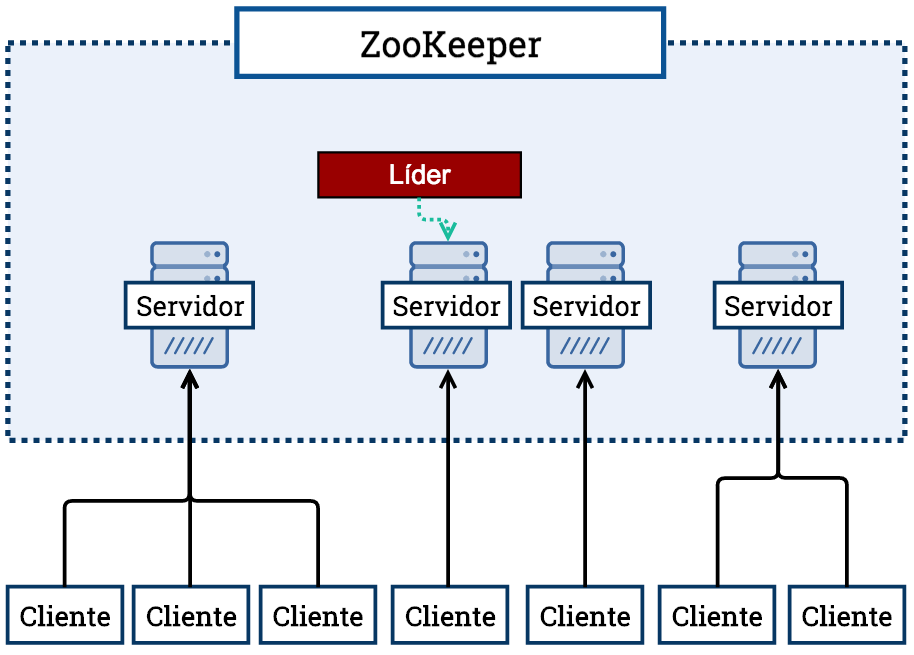
\includegraphics[scale=0.44]{servico_zookeeper.png}
	\caption{Modelo de serviço utilizado no ZooKeeper (adaptado de [59]).}
	\label{fig:servico_zookeeper}
\end{figure}

Com relação aos dados mantidos no ZooKeeper, eles são dispostos em estruturas chamadas \textbf{\textit{znodes}}, e estes podem ser comparados à arquivos e diretórios dentro de um sistema de arquivos tradicional. 

Ao contrário de um sistema de arquivo comum, que é projetado para o armazenamento dos dados, as informações gravadas no ZooKeeper são pequenos (armazenamento máximo limitado à 1 Megabyte) e são mantidos na memória, o que faz com que ele atinja uma baixa latência e altas taxas de transferência. Assim como os servidores coordenados pelo ZooKeeper são replicados para garantir a tolerância à falhas, seu próprio serviço também é replicado em diversas máquinas, a fim de se manter sempre ativo, independente de quedas e falhas. 

As máquinas coordenadas (clientes) conectam-se a um único servidor ZooKeeper. O cliente mantém uma conexão TCP na qual envia requisições, recebe respostas e envia \textbf{\textit{heartbeats}}, que são notificações periódicas enviadas do cliente ao servidor para avisá-lo que está \textit{online}, e, caso o tempo de resposta ultrapasse um determinado \textit{timeout} (configurado como 2 segundos no ZooKeeper), o servidor assume que o cliente está \textit{offline}. No caso de queda da conexão TCP entre o cliente e o servidor, o cliente tentará se conectar a outro servidor. 

O espaço de nomes implementado pelo ZooKeeper é muito parecido com o de um sistema de arquivos padrão, ou seja, um caminho absoluto é uma sequência de de caminhos relativos separados por uma barra (/). Cada nó no do espaço de nomes do ZooKeeper é identicado por um caminho. A Figura \ref{fig:estrutura_zookeeper} mostra um exemplo de uma possível estrutura hierárquica de \textit{znodes} do ZooKeeper.

\begin{figure}[H]
	\centering
	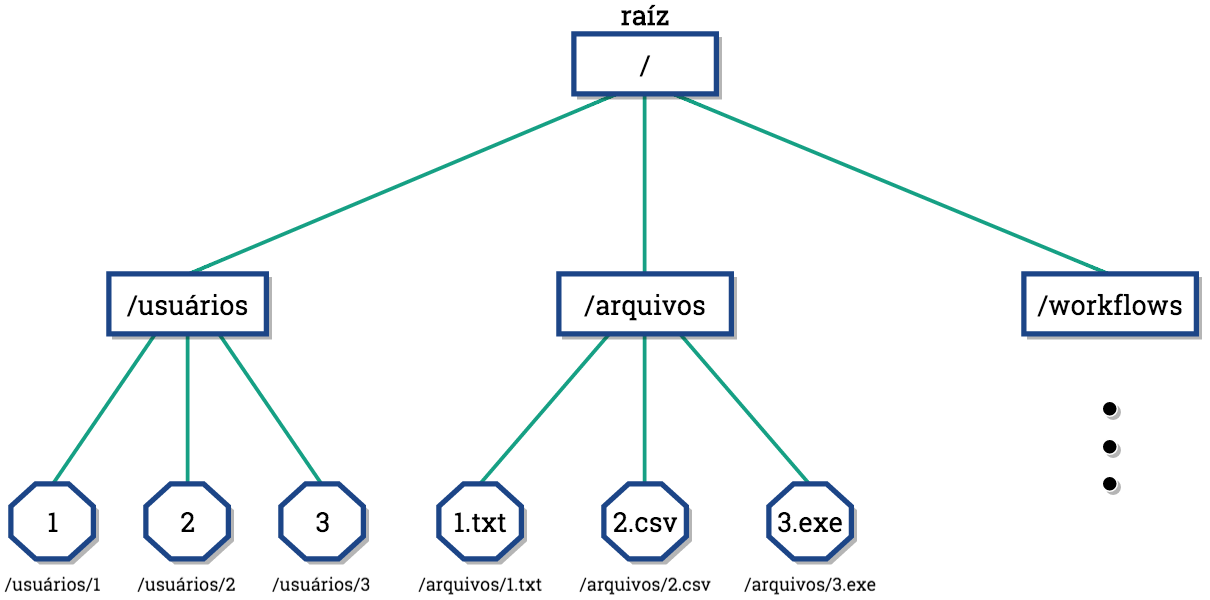
\includegraphics[scale=0.35]{estrutura_zookeeper.png}
	\caption{Exemplo de estrutura de nós do ZooKeeper.}
	\label{fig:estrutura_zookeeper}
\end{figure}

Com relação à notificação de eventos aos clientes, o ZooKeeper implementa o conceito de \textbf{\textit{watchers}}. Um \textit{watcher} é um aviso e serve para notificar alguma entidade do sistema que um \textit{znode} foi alterado. Dessa forma, para que essa entidade possa notar uma atualização em um \textit{znode}, é necessário adicionar um \textit{watcher} à ele. Assim, dada uma alteração em um nó, apenas quem inseriu um \textit{watcher} nele será notificado.

Soma-se às características apresentadas, o fato de o mesmo apresentar uma interface de programação (\textit{API - Application Programming Interface}) muito compacta, suportando operações simples, como:

\begin{itemize}
	\item \textbf{\textit{create}:} Cria um \textit{znode} na estrutura do ZooKeeper;
    \item \textbf{\textit{delete}:} Exclui um \textit{znode};
    \item \textbf{\textit{getData}:} Obtém os dados de um \textit{znode};
    \item \textbf{\textit{setData}:} Grava dados em um \textit{znode};
    \item \textbf{\textit{getChildren}:} Recupera uma lista contendo os nós filhos de um determinado \textit{znode};
    \item \textbf{\textit{exists}:} Verifica a existência de um nó dado um caminho.
\end{itemize}

Devido às características apresentadas anteriormente, o ZooKeeper então foi escolhido para coordenar os serviços e processos da plataforma BioNimbuZ.

Na Seção \ref{cap4sec2} será apresentada a arquitetura do BioNimbuZ anterior ao desenvolvimento do sistema gerenciador de \textit{workflows} científicos, objetivo do presente trabalho.

\section{Arquitetura do BioNimbuZ} \label{cap4sec2}

A arquitetura apresentada nesta Seção representa a antiga arquitetura do BioNimbuZ. Uma nova arquitetura foi proposta no presente trabalho e será apresentada e descrita no \refCap{capitulo5}. 

O BioNimbuZ utilizava uma arquitetura hierárquica, conforme mostrado na Figura \ref{fig:antiga_arquitetura} e possuía três camadas principais: interface, núcleo e infraestrutura, todas gerenciadas pelo ZooKeeper. Suas principais responsabilidades eram as seguintes:

\begin{figure}[H]
	\centering
	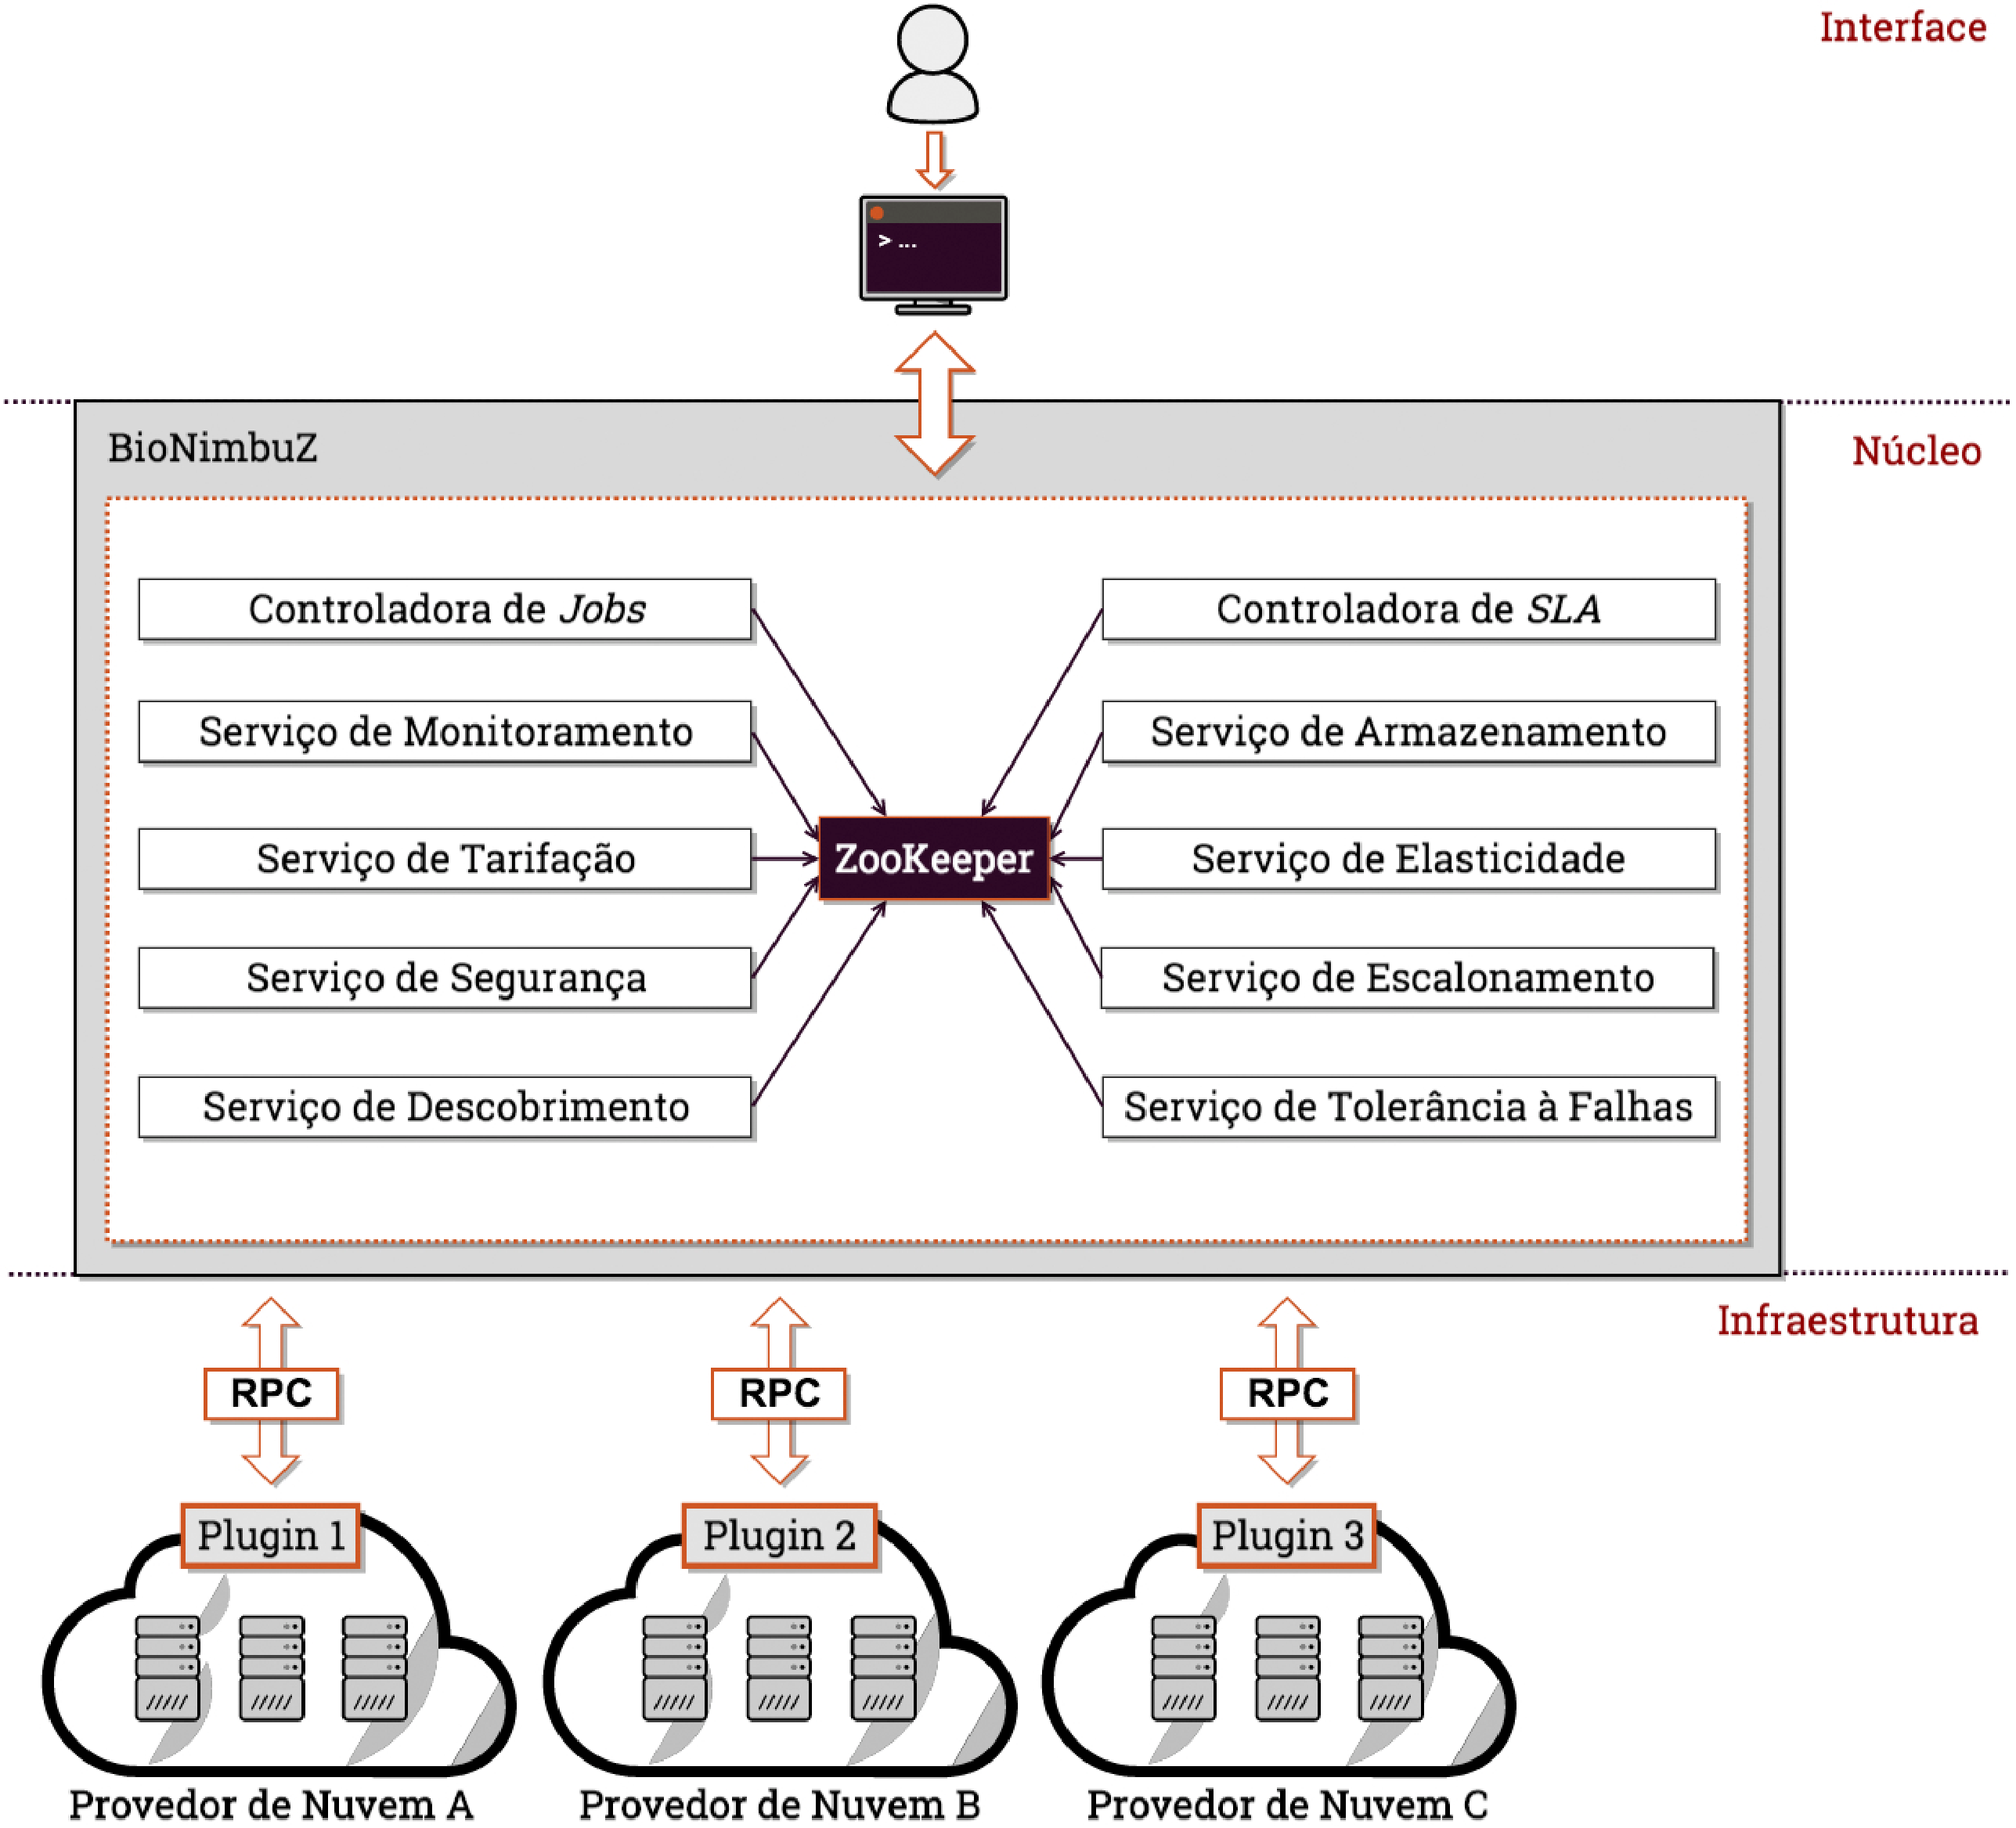
\includegraphics[scale=0.345]{antiga_arquitetura.pdf}
	\caption{Antiga arquitetura do BioNimbuZ.}
	\label{fig:antiga_arquitetura}
\end{figure}

\begin{itemize}
	\item \textbf{Camada de interface com o usuário:} Seu principal objetivo era controlar a interação com o usuário, recebendo e processando seus comandos (utilizando um \textit{terminal}) e repassando-os ao núcleo para que fossem devidamente executados;
    \item \textbf{Camada de Núcleo:} Responsável por gerenciar todos os serviços presentes na plataforma (os quais serão descritos na Seção \ref{cap4sec2subsec2}) e também por gerir toda a federação de nuvens utilizada pelo BioNimbuZ.
    \item \textbf{Camada de Infraestrutura:} Sua principal responsabilidade é prover uma interface de comunicação entre o BioNimbuZ e os provedores de nuvens. Consiste em todos os recursos computacionais que os provedores colocam à disposição da federação somados aos seus respectivos \textit{plugins} de integração.
\end{itemize}

As Seções \ref{cap4sec2subsec1}, \ref{cap4sec2subsec2} e \ref{cap4sec2subsec3} descrevem os detalhes específicos das camadas apresentadas até aqui.

\subsection{Camada de interface com o usuário} \label{cap4sec2subsec1}

Camada responsável por interagir com o usuário, recebendo seus comando e devolvendo o resultado do processamento realizado pelo núcleo, podendo ser desenvolvida de diversas maneiras: páginas \textit{web}, linhas de comando, interfaces gráficas, sistemas gerenciadores de \textit{workflows}, etc. Para tal, esses serviços de interação precisam conectar-se à Internet e se comunicar com a camada abaixo da arquitetura, o núcleo do BioNimbuZ. 

Os comandos enviados para o núcleo podiam realizar uma série de tarefas, tais como: listas os arquivos armazenados na federação, realizar o \textit{upload} de arquivos, submeter um \textit{job} para ser executado, etc. Assim, nota-se que essa camada era responsável por mostrar ao usuário uma forma de se comunicar com o BioNimbuZ.

\subsection{Camada de Núcleo} \label{cap4sec2subsec2}

Esta camada tem a atribuição de agregar os serviços providos pelo BioNimbuZ, servir como núcleo processador dos comandos provenientes da camada acima (camada de interface com o usuário, descrito na Seção \ref{cap4sec2subsec1}) e gerenciar a infraestrutura de federação de nuvens, que é a camada abaixo (camada de infraestrutura, descrita na Seção \ref{cap4sec2subsec3}).

O chamado Núcleo do BioNimbuz possuía oito serviços principais: serviço de descobrimento, serviço de monitoramento, serviço de tolerância a falhas, serviço de escalonamento, serviço de segurança, serviço de armazenamento, serviço de elasticidade e serviço de tarifação. Além destes, possuía mais duas controladoras: controladora de \textit{jobs} e controlador de \textit{SLA}. A fim de exercerem suas funcionalidades, os serviços e as controladoras interagiam entre si por meio do gerenciamento de troca de mensangens provido pelo ZooKeeper. No que tange aos serviços e controlaoras, abaixo segue uma descrição de suas respectivas funções. \\

\noindent
\textbf{\textit{Controladora de \textit{Jobs}}} \\

\noindent
É responsável por fazer a ligação entre a camada de interface com o usuário e o núcleo do BioNimbuZ. Realiza o controle de acesso dos usuários ao submeter \textit{jobs} aos recursos disponíveis na federação controlada pelo BioNimbuZ. Para realizar a verificação das credenciais do usuário, a Controladora de \textit{Jobs} acessa o Serviço de Segurança. Além disso, a Controladora de \textit{Jobs} é responsável por gerenciar os pedidos dos varios usuários, de forma a fazer o controle por usuário, mantendo os resultados para posterior consulta. \\

\noindent
\textbf{\textit{Controladora de SLA}} \\

\noindent
Atualmente, há um esforço muito grade por parte dos provedores de nuvens computacionais para que a qualidade dos serviços (\textit{Quality of Service}) prestados percebidos pelo usuário sejam os melhores possíveis. E isso apenas é possível a partir de acordos de níveis de serviço (\textit{Service Level Agreement}) assinados entre os usuários e os provedores. 

Nesse contexto, o BioNimbuZ também tem essa preocupação com a qualidade dos serviços prestados aos seus usuários. Assim, quando um usuário submete um \textit{job} para ser executado pela federação do BioNimbuZ, por meio da interface com o usuário, ele deve preencher um \textit{template} de SLA, que representa, entre outras coisas, os parâmetros de \textit{QoS} desejados pelo usuário. Estes parâmetros podem descrever desde requisitos funcionais, como número de núcleos de CPU, tamanho de memória, tamanho de armazenamento, até requisitos não funcionais, como custo a pagar e taxa de transferência.

Portanto, a Controladora de SLA tem a responsabilidade de verificar se os requisitos especificados no \textit{template} preenchido pelo usuário podem ser suportados pela federacão de nuvens naquele dado momento e, para isso, a controladora utiliza os dados de SLA informados pelo \textit{plugin} de integracão de cada provedor. \\

\noindent
\textbf{\textit{Serviço de Tolerância à Falhas}} \\

\noindent
Em ambientes de computacão em nuvem, falhas em máquinas são fatos comuns e ocorrem com frequência. Logo, uma federação de nuvens deve sempre levar em consideracão requisitos de tolerância à falhas e desenvolvimento de ambientes de alta disponibilidade.

O Serviço de Tolerância à Falhas tem como objetivo principal garantir que todos os serviços do BioNimbuZ estejam sempre disponíveis, e em caso de falhas, inicie alguma ação de recuperação. Essa recuperação exige que todos os componentes do sistema que foram afetados pela falha voltem ao seu estado anterior. O serviço de tolerância a falhas deve atuar de forma distribuída na plataforma, e estar presente em outros serviços, monitorando seu estado. 

No Serviço de Armazenamento, por exemplo, quando um alerta de indisponibilidade de um recurso é lançado por um \textit{watcher}, é iniciada uma rotina de recuperação para os arquivos que este recurso continha. Como os arquivos são replicados na federação, a recuperação ocorre de forma a identificar quais réplicas foram perdidas, realizando uma nova duplicação em outro servidor do BioNimbuZ. A tolerância à falhas no BioNimbuZ está intimamente ligada aos \textit{watchers} do ZooKeeper, pois são estes que disparam os alertas de indisponibilidade, notificando o sistema sobre problemas em algum recurso da federação.\\

\noindent
\textbf{\textit{Serviço de Escalonamento}} \\

\noindent
É o serviço responsável por receber o pedido de execução de algum \textit{job} e distribuí-las dinamicamente para os provedores disponíveis, dividindo-as em instâncias menores - chamadas \textit{tasks}. O serviço de escalonamento também é responsável por acompanhar toda a execução de um \textit{job}, e manter um registro das execuções já escalonadas. 

Para realizar a distribuição de tarefas na federação, algumas métricas são levadas em consideração, como latência, balanceamento de carga, tempo de espera e capacidade de processamento dos recursos disponíveis, entre outras, visando atender o que foi determinado no acordo de SLA. \\

\noindent
\textbf{\textit{Serviço de Sergurança}} \\

\noindent
Segurança em nuvens federadas é uma área de estudo em constante evolução, e este serviço deve trabalhar em diversos pontos para fornecer um serviço efetivamente seguro, mitigando possíveis pontos de falhas no sistema. 

Dois pontos constituem o cerne deste serviço: autenticação e autorização. O primeiro, está focado em saber se o usuário que está tentando acessar algum recurso na federação é quem ele realmente diz ser. Depois de estar autenticado no sistema, o segundo passo é a autorização, que consiste em verificar se o usuário pode realizar aquela ação que está demandando. 

Muitos outros aspectos podem ser abordados por este serviço, como a criptografia de mensagens, para garantir a confidencialidade na troca de informações entre provedores, por exemplo, e também a verificação de integridade de arquivos, de modo que seja possível garantir que um arquivo não seja alterado por fatores externos à federação, como por exemplo um componente de rede gerando erros nos dados trafegados. \\

\noindent
\textbf{\textit{Serviço de Armazenamento}} \\

\noindent
Responsável pela estratégia de armazenamento dos arquivos que são utilizados ou mantidos pelo BioNimbuZ, o serviço deve decidir sobre a distribuição dos arquivos entres os diferentes provedores da federação. Para isso, o serviço de armazenamento comunica-se com o serviço de descobrimento para obter acesso as informações sobre a federação. Com isso, o serviço saberá as condições atuais de armazenamento de cada um dos provedores que faz parte da federação.

O armazenamento deve ocorrer de forma eficiente, para que as aplicações possam utilizar os arquivos com o menor custo possível. Este custo é calculado utilizando-se algumas métricas, tais como, latência de rede, distância entre os provedores e capacidade de armazenamento. Também é adotada a replicação dos arquivos em mais de um provedor, também visando a diminuição de custos envolvidos. \\

\noindent
\textbf{\textit{Serviço de Elasticidade}} \\

\noindent
Sua função é, dinamicamente, aumentar ou diminuir o poder computacional total da federação. Para tal, gera novas instâncias ou desliga instâncias ociosas de máquinas virtuais, ou então reajusta as configurações de CPU, de memória, de largura de banda, entre outros recursos que são disponibilizados pelos provedores de nuvem, a fim de se obter uma melhor utilização da infraestrutura disponível. 

A elasticidade pode ser vertical, quando há um redimensionamento das configurações da máquina virtual, como também pode ser horizontal, quando é altera-se o número de máquinas virtuais instanciadas nos provedores. \\

\noindent
\textbf{\textit{Serviço de Tarifação}} \\

\noindent
Tem a responsabilidade de calcular o quanto os usuários devem pagar pela utilização dos serviços oferecidos na plataforma BioNimbuZ. Para que isto seja possível, este serviço se mantém em constante contato com o serviço de monitoramento, para obter informações, tais como tempo de execução e quantidade de máquinas virtuais alocadas das tarefas que foram executadas por determinado usuário. Dessa forma é possível verificar quais recursos foram alocados para determinada carga de trabalho submetida pelo usuário, obtendo-se assim, o preço devido.\\ 

\noindent
\textbf{\textit{Serviço de Descobrimento}} \\

\noindent
Responsável por identificar e manter informações como poder computacional, capacidade de armazenamento e latência de rede, à respeito dos provedores de nuvem presentes na federação. Também mantém detalhes sobre parâmetros de execução e arquivos de entrada e de saída dos softwares disponíveis para execução pelo usuário. 

Toda vez que um provedor é incluído na federação de nuvens, seus dados são gravado em um novo \textit{znode} no ZooKeeper. Assim, para qualquer outro serviço obter informações acerca dos provedores presentes na federação, basta realizar uma consulta simples no ZooKeeper. Sempre que as informações acerca de um provedor são atualizadas (por exemplo com a diminuição do poder computacional ou falta de espaço de armazenamento), outros serviços são notificados, a partir dos \textit{watchers} que foram adicionados. Dessa forma, todo o sistema tem acesso à essas informações.\\ 

\noindent
\textbf{\textit{Serviço de Monitoramento}} \\

\noindent
Este serviço monitora a nuvem federada verificando as aplicações e os \textit{jobs} para a execução. Ao receber um pedido de execução de um \textit{job}, vindo da Controladora de \textit{Jobs}, o Serviço de Monitoramento identica se o software computacional relacionado àquele \textit{job} está disponível em algum provedor de serviço, e então redireciona o pedido para o Serviço de Escalonamento, o qual processa o pedido garantindo que todas as requisições sejam devidamente atendidas e executadas. 

A fim de retribuir informações acerca da execução das tarefas, mensagens periódicas são enviadas para os recursos gerenciados pelo BioNimbuZ. Além disso, notifica a Controladora de \textit{Jobs} sobre o estado da execução de determinado \textit{Job}.

Dessa forma, é por meio dessas mensagens periódicas que o Serviço de Monitoramento é capaz de vericar se uma execução é finalizada com sucesso sem violar os parâmetros de SLA acordados com o usuário.

\noindent
\subsection{Camada de Infraestrutura} \label{cap4sec2subsec3}
 
A camada de infraestrutura consiste nos recursos computacionais disponibilizados na federação por meio dos provedores de nuvem, visíveis ao BioNimbuz através dos \textit{plugins} de integração. Essa camada provê meios para que haja a comunicação entre o BioNimbuZ e os provedores presentes na federação, mapeando os comandos vindos da arquitetura do BioNimbuZ para comandos específicos de cada provedor.

 

	



